\documentclass[14pt, fleqn, xcolor={dvipsnames, table}]{beamer}
\usepackage[T2A]{fontenc}
\usepackage[utf8]{inputenc}
\usepackage[english,russian]{babel}
\usepackage{amssymb,amsfonts,amsmath,mathtext}
\usepackage{cite,enumerate,float,indentfirst}
\usepackage{cancel}
\usepackage{graphicx}
\usepackage{animate}

\usepackage{tikz}
% \usepackage{enumitem}
\usetikzlibrary{shadows}

% \usepackage{enumitem}
% \setitemize{label=\usebeamerfont*{itemize item}%
%   \usebeamercolor[fg]{itemize item}
%   \usebeamertemplate{itemize item}}

\graphicspath{{images/}}

\usetheme{Madrid}
\usecolortheme{seahorse}
\renewcommand{\CancelColor}{\color{red}}

\setbeamercolor{footline}{fg=Blue!50}
\setbeamertemplate{footline}{
  \leavevmode%
  \hbox{%
  \begin{beamercolorbox}[wd=.333333\paperwidth,ht=2.25ex,dp=1ex,center]{}%
    И. Кураленок, Н. Поваров, Яндекс
  \end{beamercolorbox}%
  \begin{beamercolorbox}[wd=.333333\paperwidth,ht=2.25ex,dp=1ex,center]{}%
    Санкт-Петербург, 2014
  \end{beamercolorbox}%
  \begin{beamercolorbox}[wd=.333333\paperwidth,ht=2.25ex,dp=1ex,right]{}%
  Стр. \insertframenumber{} из \inserttotalframenumber \hspace*{2ex}
  \end{beamercolorbox}}%
  \vskip0pt%
}
\newcommand\indentdisplays[1]{%
     \everydisplay{\addtolength\displayindent{#1}%
     \addtolength\displaywidth{-#1}}}
\newcommand{\itemi}{\item[\checkmark]}

\newenvironment{mydescription}[1]
  {\begin{list}{}%  
   {\renewcommand\makelabel[1]{\color{blue}##1:\hfill}%
   \settowidth\labelwidth{\makelabel{#1}}%
   \setlength\leftmargin{\labelwidth}
   \addtolength\leftmargin{\labelsep}}}
  {\end{list}}

\title{Нейронные сети\\\small{совсем чуть-чуть}}
\author[]{\small{%
И.~Куралёнок,
Н.~Поваров}}
\date{}
\begin{document}

\begin{frame}
\maketitle
\small
\begin{center}
\vspace{-60pt}
\normalsize {\color{red}Я}ндекс \\
\vspace{80pt}
\footnotesize СПб, 2014
\end{center}
\end{frame}
\section{Постановка задачи и виды} % про сведение решающей функции к комбинации зависимых переменных инженерным способом

\begin{frame}{Постановка задачи обучения}{}
{\color{blue}С построением фичей}: повесим на клиента датчики \\
\textit{Наша цель повесить датчики правильно, зная какую информацию мы хотим получить.}\\
Похоже на glass box\\
~\\
{\color{blue}Без построения фичей}: льется поток неведомых данных \\
\textit{Хотим выделить сигналы, имеющие отношение к искомому} \\
Похоже на black box
\end{frame}

\begin{frame}{Пример с милиционером и бабушкой}

\end{frame}

\begin{frame}{Немного рассуждений}
\small
\textbf{А можно ли одновременно оптимизировать и выделение полезной информации и обучение?}\\
\begin{itemize}
\uncover<2->{\item Ограничимся линейными моделями как в решающей функции, так и в построении FE}
\only<2>{$$
F = \sum_i w_i \left(v_i^T x\right) 
$$}
\uncover<3->{\item Но так все сведется к линейной регрессии! Давайте добавим какое-нибудь нелинейное преобразование}
\only<3>{$$
F = \sum_i w_i g\left(v_i^T x\right)
$$}
\uncover<4->{\item Если преобразование монотонное, то можно его для красоты применить и к результату}
\only<4>{$$
F = g\left(\sum_i w_i g\left(v_i^T x\right)\right)
$$}
\uncover<5->{\item Дополним рекурсией и будем подбирать не одну функцию а несколько}
\only<5->{$$
F_i = g\left(\mathbf{w}_{di}^T g(W_{d-1}g(\ldots g(W_{0}x))\right)
$$}
\end{itemize}
\uncover<6->{$\Rightarrow$Понятно, что так писать не удобно.}
\end{frame}

\begin{frame}{Персептрон Розенблатта}
\small
$$
F_i = g\left(\mathbf{w}_{di}^T g(W_{d-1}g(\ldots g(W_{0}x))\right)
$$
Как можно видеть, система состоит из некоторого количества блоков $g(W_tu)$. Если блок 1, $g = sign(x)$ и мы подбираем одну функцию, то
\begin{center}
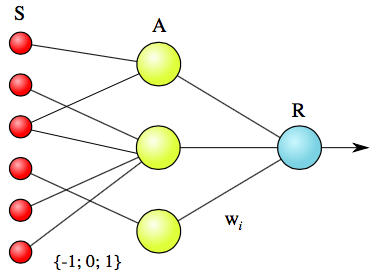
\includegraphics[width=0.4\textwidth]{Simple_perceptron}
\end{center}
это элементарный персептрон Розенблатта. Если блоков много, то сложный :).
\end{frame}

\section{Биология и основные понятия} % подробно про функции разных кусков
\begin{frame}{}
\begin{center}
\Huge
Но на самом деле все было не так!\\
~\\
\small
\uncover<2->{
\textbf{Искусственные нейронные сети (ИНС)} --- математические модели, а также их программные или аппаратные реализации, построенные по принципу организации и функционирования биологических нейронных сетей --- сетей нервных клеток живого организма.
}
\end{center}
\end{frame}

\begin{frame}{Нейрон I}
\begin{center}
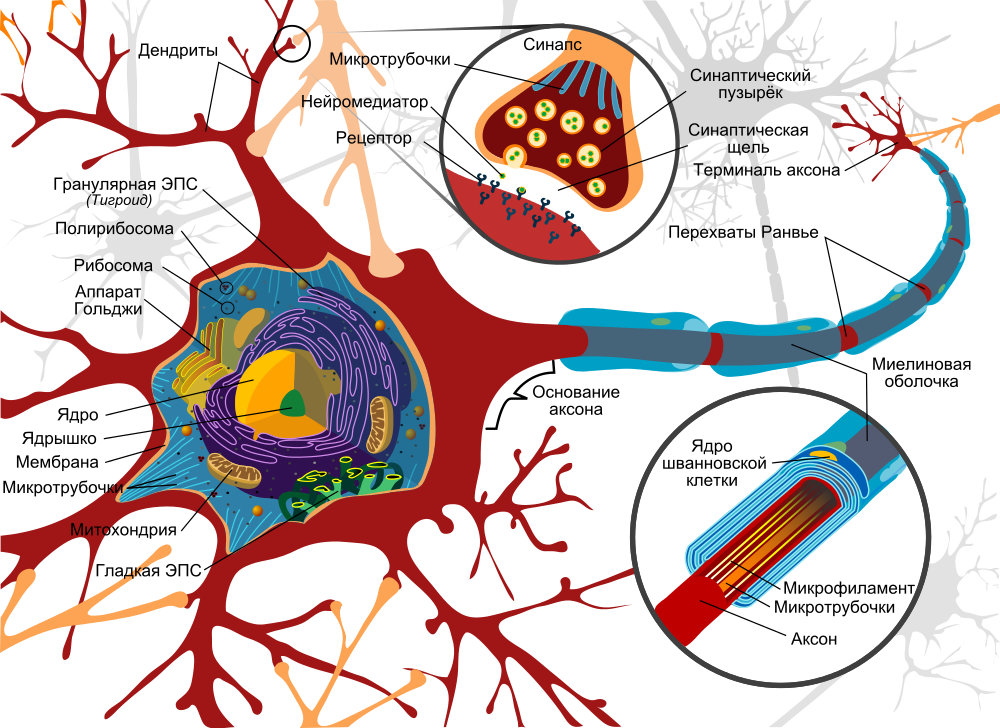
\includegraphics[width=0.8\textwidth]{normal_neuron}
\end{center}
\end{frame}

\begin{frame}{Нейрон II}
\begin{center}
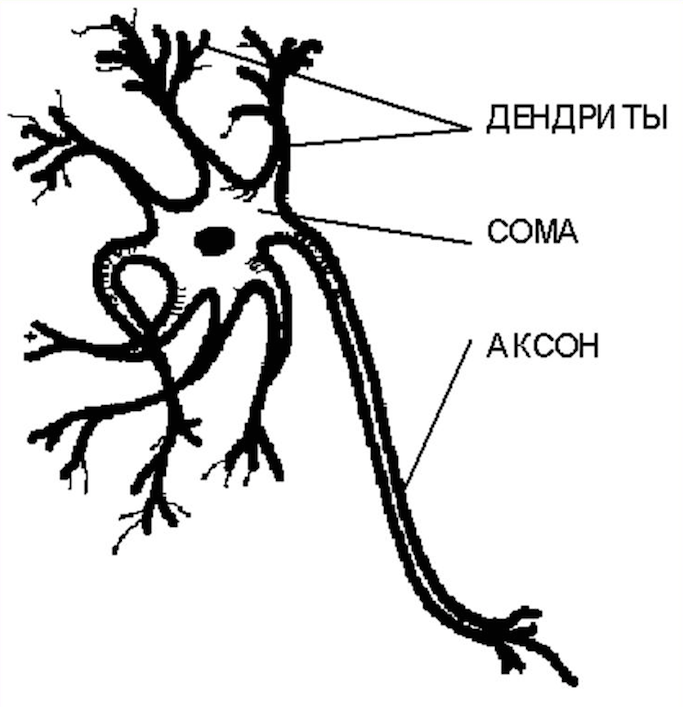
\includegraphics[width=0.6\textwidth]{neuron_simple}
\end{center}
\end{frame}

\begin{frame}{Карго I}
\begin{center}
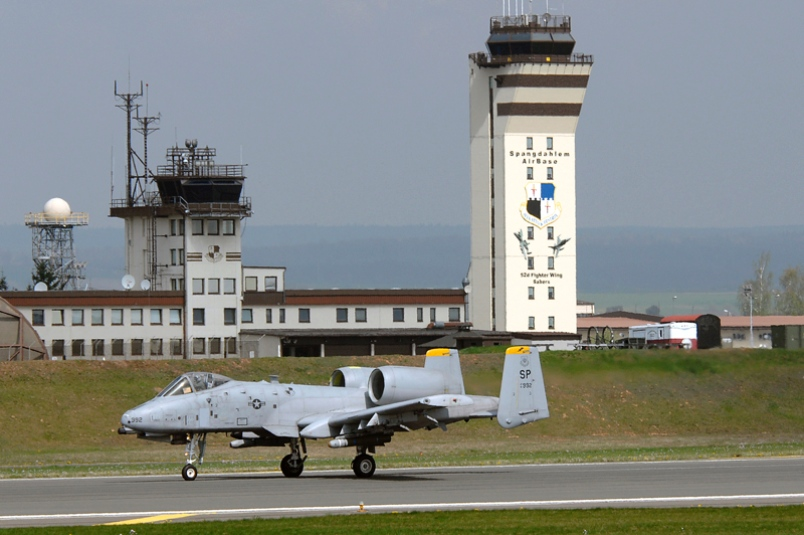
\includegraphics[width=0.9\textwidth]{good_cargo}
\end{center}
\end{frame}


\begin{frame}{Карго II}
\begin{center}
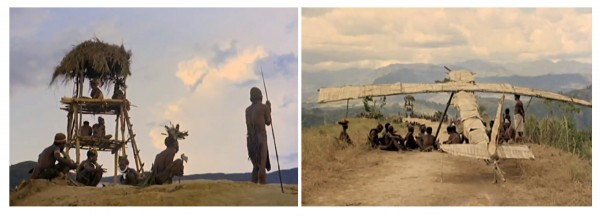
\includegraphics[width=0.9\textwidth]{cult_cargo}
\end{center}
\end{frame}

\begin{frame}{Немного истории}
\begin{enumerate}
  \item McCulloch, Pitts. ``A Logical Calculus of Ideas Immanent in Nervous Activity''. 1943
  \item ``Кибернетическая модель мозга'' 1957
  \item ЭВМ Mark I 1960
  \item Minsky, Papert ``Perceptrons: an introduction to computational geometry'' 1969
  \item ЭВМ Mark III 1985
  \item Google Brain vs. Котики 2011 (Andrew Ng and co.)
  \item Krizhevsky, A., Sutskever, I. and Hinton, G. E. ``ImageNet Classification with Deep Convolutional Neural Networks'' 2012
\end{enumerate}

\end{frame}

\begin{frame}{Отличия от машин фон Неймана}
\begin{itemize}
  \item Массовый параллелизм;
  \item Распределённое представление информации и вычисления
  \item Способность к обучению и обобщению
  \item Адаптивность
  \item Свойство контекстуальной обработки информации
  \item Толерантность к ошибкам
  \item Низкое энергопотребление
\end{itemize}
\end{frame}

\begin{frame}{Типы нейро компьютеров}
\begin{center}
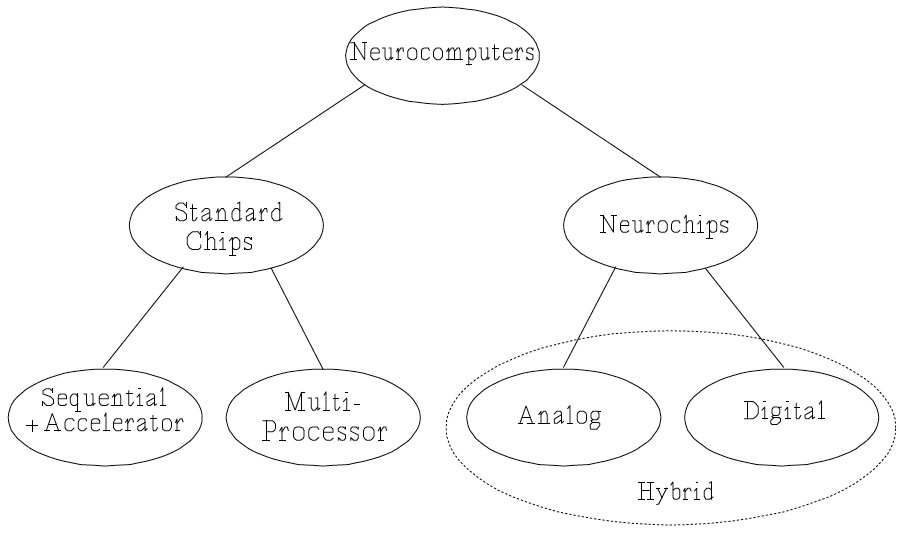
\includegraphics[width=0.8\textwidth]{neurocomp-types}
\end{center}
\end{frame}

\begin{frame}{Виды нейронных сетей}
По числу слоев:
\begin{itemize}
  \item Однослойные 
  \item Двухслойные
  \item Многослойные
\end{itemize}

По способу взаимодействия нейронов:
\begin{itemize}
  \item C обратной связью
  \item Без обратной связи
  \item По нескольким соседям
\end{itemize}
\end{frame}

\begin{frame}{Известные типы сетей}
\begin{itemize}
  \item Персептронные сети
  \item Ассоциативная память
  \item SOM
  \item etc.
\end{itemize}
\end{frame}

\section{Персептронные сети и обратное распространение ошибки}

\begin{frame}{Персептрон Розенблатта}
\small
$$
F_i = g\left(\mathbf{w}_{di}^T g(W_{d-1}g(\ldots g(W_{0}x))\right)
$$
Как можно видеть, система состоит из некоторого количества блоков $g(W_tu)$. Если блок 1, $g = sign(x)$ и мы подбираем одну функцию, то
\begin{center}
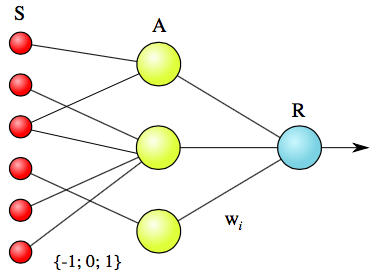
\includegraphics[width=0.4\textwidth]{Simple_perceptron}
\end{center}
это элементарный персептрон Розенблатта. Если блоков много, то сложный :).\\
\textbf{Без обратной связи, многослойная}
\end{frame}

\begin{frame}{Обучение персептронной сети}{Обратное распространение ошибки}
\footnotesize
С $sign$ работать тяжело, поэтому возьмем $g$ поглаже ($th, \frac{1}{1+e^{-t}}$, etc.), тогда можно сделать стохастический градиентный спуск, воспользовавшись блочной структурой решающей функции:
$$
\arg \max_{\{W_l\}} T(y, F(x, \{W_l\}_1^d)) = \arg\max_{\{W_l\}} T(y, g(W_l y_{l-1}))
$$
\begin{itemize}
  \item Посчитаем частные производные для выходного слоя:
  $$
  w_{ij}^{dt+1} = w_{ij}^{dt} - \frac{\partial T}{\partial y_i^d}\frac{\partial g}{\partial w_{ij}^d}\left(\{W^t\}_1^d\right)
  $$
  \item Для предпоследнего слоя:
  $$
  w_{ij}^{d-1t+1}  = w_{ij}^{d-1t+1} - \left(\sum_k \frac{\partial T}{\partial y_k^d}\frac{\partial T}{\partial y_j^{d-1}}\right)\frac{\partial g}{\partial w_{ij}^{d - 1}}\left(\{W^t\}_1^d\right)
  $$
  \end{itemize}
\end{frame}

\begin{frame}{Обратное распространение ошибки в случае MSE}
\footnotesize
Нам интересно научиться строить регрессию.
$$\begin{array}{c}
T = -\frac{1}{2}\|y - F(x, \{W_l\}_1^d)\|^2 \\
g(u) = \frac{1}{1 + e^{-u}}
\end{array}$$


\begin{itemize}
  \item Посчитаем частные производные для выходного слоя:
  \only<-2>{$$
  w_{ij}^{dt+1} = w_{ij}^{dt} - \frac{\partial T}{\partial y_i^d}\frac{\partial g}{\partial w_{ij}^d}\left(\{W^t\}_1^d\right)
  $$}
  \only<2->{
  $$
  w_{ij}^{dt+1} = w_{ij}^{dt} - y_i^{d-1}y_j^d(1 - y^d_j)(y_j^d - y)
  $$}
  \item Для предпоследнего слоя:
  \only<-3>{$$
  w_{ij}^{d-1t+1}  = w_{ij}^{d-1t+1} - \left(\sum_k \frac{\partial T}{\partial y_k^d}\frac{\partial T}{\partial y_j^{d-1}}\right)\frac{\partial g}{\partial w_{ij}^{d - 1}}\left(\{W^t\}_1^d\right)
  $$
  }
  \only<3->{
  $$
  w_{ij}^{d-1t+1} = w_{ij}^{d-1t+1} + y_i^{d-2}y_j^{d - 1}\left(1 - y_j^{d-1}\right)\sum_k w_{jk}^{dt}y_k^d(1 - y^d_k)(y^d_k - y)
  $$}
\end{itemize}
\end{frame}

% понятие персептрона, BP, расширения персептронных сетей W-нейроны и прочая херня

\section{Ассоциотивная память} % Сети Хопфилда, Bolzman machine
\begin{frame}{Сети Хопфилда}{Авто-ассоциативная память}
\footnotesize
\begin{center}
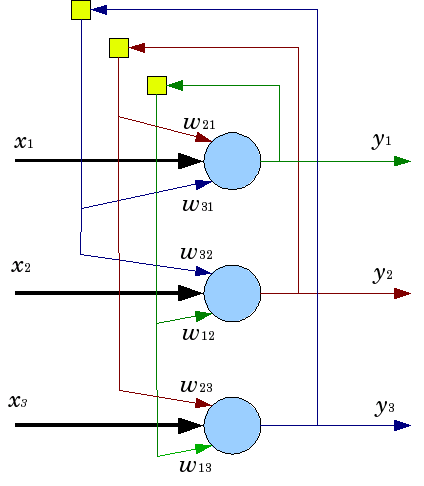
\includegraphics[height=0.4\textheight]{Hopfield_net}
\end{center}
\begin{itemize}
  \item Подадим сигнал на входы $x = \{-1,1\}^n$
  \item Подождем пока они по закону $x^{t+1} = -1^{sign(Wx^t - \theta)}$
  \item Узнаем какие код решения
\end{itemize}
\textbf{С обратной связью, однослойная}
\end{frame}

\begin{frame}{Обучение сетей Хопфилда}
\small
На самом деле, мы знаем куда это добро сойдется, если подать заданный сигнал $x$
$$
\arg \min_{u_0 = x}\footnote{При фиксированной выше процедуре оптимизации (конвергенции), которая даже сходится в асинхронном случае} E(u) = \arg \min_{u_0 = x} -\frac{1}{2}u^T W u + \theta^Tu
$$
мы дойдем до \textit{локального} минимума, которых может быть много в зависимости от $W$. Если:
$$
W = \frac{1}{m}\sum_{k=1}^m x_k x^T_k
$$
то минимумы будут именно в этих точках. 
\end{frame}

\begin{frame}{Свойства сетей Хопфилда}
\begin{itemize}
  \item Не думают, а скорее реализуют адаптивную функцию ближайшего соседа
  \item Сходятся, имеют эффективную параллельную реализацию
  \item Могут работать долго и в результате дать ``химеру''
\end{itemize}
\end{frame}

\begin{frame}{Как ту же идею заставить ``думать''}{Bolzmann machine}
\footnotesize
Немного поменяем как все это добро работает: сделаем значения в нодах из $\{0,1\}$, договоримся о 0-х на диагонали $W$. Будем надеяться, что состояния системы распределены по Больцману:
$$
p(s|W,\theta) \sim e^{s^T W s + \theta^Ts \over kT}
$$
Тогда веса $W$ и $\theta$ мы можем исходя из близости этого распределения и того, которое хотим получить:
$$
\arg\min_{W,\theta} \sum_s p(s|X) log \frac{p(s|X)}{p(s|W)}
$$
Отдельно рассматривают ограничение на связи внутри думающего (hidden) уровня, такое называют RBM.\\
\textbf{С обратной связью, двухслойная}
\end{frame}


\begin{frame}{Что мы сегодня узнали}
\begin{itemize}
  \item Можно решать задачи обучения в комплексе
  \item Есть прямые аналогии в биологии (культ карго) и этим пробовали пользоваться
  \item Это сложно (получается при большой удаче) и для этого есть специальный язык
  \item Есть разные принципы построения взаимодействия внутри сети
  \item Природа все равно без датчиков не живет
\end{itemize}
\end{frame}
\end{document}
